\documentclass[runningheads]{llncs}

\usepackage[review,year=2026,ID=*****]{eccv}
\usepackage{eccvabbrv}
\usepackage{graphicx}
\usepackage{booktabs}
\usepackage{subcaption}
\usepackage{amsmath}

\usepackage{listings}
\lstdefinestyle{prompt}{
  basicstyle=\ttfamily\footnotesize,
  breaklines=true, breakindent=0pt,
  columns=fullflexible, keepspaces=true,
  frame=single, framesep=4pt, xleftmargin=2pt,
}


\usepackage{newunicodechar}
\newunicodechar{°}{\ensuremath{^\circ}}\newunicodechar{×}{\ensuremath{\times}}\newunicodechar{–}{--}\newunicodechar{—}{---}
\newunicodechar{↔}{\ensuremath{\leftrightarrow}}\newunicodechar{δ}{\ensuremath{\delta}}\newunicodechar{α}{\ensuremath{\alpha}}
\newunicodechar{≈}{\ensuremath{\approx}}\newunicodechar{→}{\ensuremath{\rightarrow}}\newunicodechar{≤}{\ensuremath{\le}}
\newunicodechar{≥}{\ensuremath{\ge}}\newunicodechar{≪}{\ensuremath{\ll}}\newunicodechar{≫}{\ensuremath{\gg}}\newunicodechar{·}{\ensuremath{\cdot}}
\newunicodechar{∈}{\ensuremath{\in}}\newunicodechar{±}{\ensuremath{\pm}}\newunicodechar{−}{\ensuremath{-}}\newunicodechar{≠}{\ensuremath{\neq}}
\newunicodechar{“}{``}\newunicodechar{”}{''}\newunicodechar{‘}{`}\newunicodechar{’}{'}\newunicodechar{Δ}{\ensuremath{\Delta}}\newunicodechar{★}{\ensuremath{\star}}\newunicodechar{∼}{\ensuremath{\sim}}\newunicodechar{Φ}{\ensuremath{\Phi}}\newunicodechar{σ}{\ensuremath{\sigma}}\newunicodechar{ρ}{\ensuremath{\rho}}\newunicodechar{θ}{\ensuremath{\theta}}\newunicodechar{ℓ}{\ensuremath{\ell}}
\newunicodechar{é}{\'e}\newunicodechar{è}{\`e}\newunicodechar{ê}{\^e}\newunicodechar{ô}{\^o}\newunicodechar{ö}{\"o}\newunicodechar{ü}{\"u}\newunicodechar{ä}{\"a}\newunicodechar{á}{\'a}\newunicodechar{ñ}{\~n}\newunicodechar{ç}{\c{c}}

\usepackage{hyperref}
% AUTO-GENERATED by scripts/emit_paper_tex.py from results/metrics/paper_data.json. DO NOT EDIT.
% git ec6ae88  config 07bca1207c0a  fast=False
\newcommand{\HumanTFPone}{0.49}
\newcommand{\HumanTFPend}{0.93}
\newcommand{\HumanNumFixTP}{3}
\newcommand{\HumanNumFixTA}{5}
\newcommand{\HumanNumFixTAmax}{45}
\newcommand{\HumanCeiling}{0.53}
\newcommand{\HumanDprime}{2.91}
\newcommand{\NImages}{285}
\newcommand{\NImagesTP}{141}
\newcommand{\NImagesTA}{144}
\newcommand{\NSeeds}{5}
\newcommand{\PCApcone}{45}
\newcommand{\PCApctwo}{30}
\newcommand{\NEpisodes}{38{,}475}
\newcommand{\QwenTPexist}{0.99}
\newcommand{\QwenTAexist}{0.81}
\newcommand{\QwenYesBias}{0.19}
\newcommand{\QwenLocaliz}{0.00}
\newcommand{\QwenSharpTFPone}{0.97}
\newcommand{\QwenSharpTFPend}{0.97}
\newcommand{\QwenSharpNumFixTP}{2}
\newcommand{\QwenSharpNumFixTA}{1}
\newcommand{\QwenSharpDeclAbs}{0.94}
\newcommand{\QwenSharpFalsePresent}{0.06}
\newcommand{\QwenSharpDprime}{3.66}
\newcommand{\QwenSharpEntropyD}{$-$.68}
\newcommand{\QwenSharpSaccD}{$+$.52}
\newcommand{\QwenSharpCenterD}{$-$.20}
\newcommand{\QwenSharpSelfConsist}{0.84}
\newcommand{\QwenSharpScanmatchAH}{0.50}
\newcommand{\QwenSharpDensityCC}{0.55}
\newcommand{\QwenGPTFPone}{0.97}
\newcommand{\QwenGPTFPend}{0.98}
\newcommand{\QwenGPNumFixTP}{2}
\newcommand{\QwenGPNumFixTA}{1}
\newcommand{\QwenGPDeclAbs}{0.93}
\newcommand{\QwenGPFalsePresent}{0.07}
\newcommand{\QwenGPDprime}{3.84}
\newcommand{\QwenGPEntropyD}{$-$.67}
\newcommand{\QwenGPSaccD}{$+$.50}
\newcommand{\QwenGPCenterD}{$-$.18}
\newcommand{\QwenGPSelfConsist}{0.84}
\newcommand{\QwenGPScanmatchAH}{0.50}
\newcommand{\QwenGPDensityCC}{0.58}
\newcommand{\QwenKsixteenTFPone}{0.78}
\newcommand{\QwenKsixteenTFPend}{0.91}
\newcommand{\QwenKtwentyfourTFPone}{0.56}
\newcommand{\QwenKtwentyfourTFPend}{0.81}
\newcommand{\QwenKthirtytwoTFPone}{0.42}
\newcommand{\QwenKthirtytwoTFPend}{0.71}
\newcommand{\QwenNumFixCIzero}{no}
\newcommand{\QwenNumFixDelta}{-1.49}
\newcommand{\GlmTPexist}{0.99}
\newcommand{\GlmTAexist}{0.81}
\newcommand{\GlmYesBias}{0.19}
\newcommand{\GlmLocaliz}{0.31}
\newcommand{\GlmSharpTFPone}{0.97}
\newcommand{\GlmSharpTFPend}{0.98}
\newcommand{\GlmSharpNumFixTP}{2}
\newcommand{\GlmSharpNumFixTA}{4}
\newcommand{\GlmSharpDeclAbs}{0.91}
\newcommand{\GlmSharpFalsePresent}{0.03}
\newcommand{\GlmSharpDprime}{4.09}
\newcommand{\GlmSharpEntropyD}{$-$.65}
\newcommand{\GlmSharpSaccD}{$+$.60}
\newcommand{\GlmSharpCenterD}{$-$.29}
\newcommand{\GlmSharpSelfConsist}{0.90}
\newcommand{\GlmSharpScanmatchAH}{0.48}
\newcommand{\GlmSharpDensityCC}{0.54}
\newcommand{\GlmGPTFPone}{0.97}
\newcommand{\GlmGPTFPend}{0.98}
\newcommand{\GlmGPNumFixTP}{2}
\newcommand{\GlmGPNumFixTA}{4}
\newcommand{\GlmGPDeclAbs}{0.91}
\newcommand{\GlmGPFalsePresent}{0.03}
\newcommand{\GlmGPDprime}{4.23}
\newcommand{\GlmGPEntropyD}{$-$.65}
\newcommand{\GlmGPSaccD}{$+$.61}
\newcommand{\GlmGPCenterD}{$-$.31}
\newcommand{\GlmGPSelfConsist}{0.91}
\newcommand{\GlmGPScanmatchAH}{0.48}
\newcommand{\GlmGPDensityCC}{0.63}
\newcommand{\GlmKsixteenTFPone}{0.71}
\newcommand{\GlmKsixteenTFPend}{0.80}
\newcommand{\GlmKtwentyfourTFPone}{0.49}
\newcommand{\GlmKtwentyfourTFPend}{0.65}
\newcommand{\GlmKthirtytwoTFPone}{0.33}
\newcommand{\GlmKthirtytwoTFPend}{0.53}
\newcommand{\GlmNumFixCIzero}{no}
\newcommand{\GlmNumFixDelta}{-1.60}
\newcommand{\GemmaTPexist}{0.97}
\newcommand{\GemmaTAexist}{0.80}
\newcommand{\GemmaYesBias}{0.20}
\newcommand{\GemmaLocaliz}{0.87}
\newcommand{\GemmaSharpTFPone}{0.80}
\newcommand{\GemmaSharpTFPend}{0.93}
\newcommand{\GemmaSharpNumFixTP}{3}
\newcommand{\GemmaSharpNumFixTA}{6}
\newcommand{\GemmaSharpDeclAbs}{0.96}
\newcommand{\GemmaSharpFalsePresent}{0.03}
\newcommand{\GemmaSharpDprime}{3.11}
\newcommand{\GemmaSharpEntropyD}{$-$.28}
\newcommand{\GemmaSharpSaccD}{$+$.24}
\newcommand{\GemmaSharpCenterD}{$+$.06}
\newcommand{\GemmaSharpSelfConsist}{0.71}
\newcommand{\GemmaSharpScanmatchAH}{0.47}
\newcommand{\GemmaSharpDensityCC}{0.49}
\newcommand{\GemmaGPTFPone}{0.80}
\newcommand{\GemmaGPTFPend}{0.93}
\newcommand{\GemmaGPNumFixTP}{3}
\newcommand{\GemmaGPNumFixTA}{5}
\newcommand{\GemmaGPDeclAbs}{0.96}
\newcommand{\GemmaGPFalsePresent}{0.02}
\newcommand{\GemmaGPDprime}{3.14}
\newcommand{\GemmaGPEntropyD}{$-$.27}
\newcommand{\GemmaGPSaccD}{$+$.23}
\newcommand{\GemmaGPCenterD}{$+$.06}
\newcommand{\GemmaGPSelfConsist}{0.71}
\newcommand{\GemmaGPScanmatchAH}{0.47}
\newcommand{\GemmaGPDensityCC}{0.50}
\newcommand{\GemmaKsixteenTFPone}{0.42}
\newcommand{\GemmaKsixteenTFPend}{0.75}
\newcommand{\GemmaKtwentyfourTFPone}{0.28}
\newcommand{\GemmaKtwentyfourTFPend}{0.65}
\newcommand{\GemmaKthirtytwoTFPone}{0.19}
\newcommand{\GemmaKthirtytwoTFPend}{0.59}
\newcommand{\GemmaNumFixCIzero}{yes}
\newcommand{\GemmaNumFixDelta}{-0.03}


\begin{document}

\title{Supplementary Material\\ Matched Outcomes, Divergent Gaze: How Foveated MLLMs Search Compared to Humans}
\titlerunning{Supplementary Material}
\author{Anonymous ECCV 2026 submission}
\authorrunning{Anonymous ECCV 2026 submission}
\institute{Paper ID *****}
\maketitle

\renewcommand{\thesection}{S\arabic{section}}
\renewcommand{\thetable}{S\arabic{table}}
\renewcommand{\thefigure}{S\arabic{figure}}
\setcounter{section}{0}\setcounter{table}{0}\setcounter{figure}{0}

This document specifies the experimental methods in full, gives formal definitions of every behavioural
measure and the statistical procedures used to analyse them, and reports the complete per-model results
summarised in the main paper. We first describe the stimuli and the foveation model
(Sec.~\ref{sec:fov}) and the search procedure (Sec.~\ref{sec:proc}); we then define all metrics and the
inferential methodology (Sec.~\ref{sec:metrics}). The three behavioural axes (decision, finding, and
gaze) are reported in Secs.~\ref{sec:decision}--\ref{sec:gaze}, followed by the multivariate analysis
(Sec.~\ref{sec:pca}), the mechanistic analyses (Sec.~\ref{sec:mech}), robustness and cross-model
variation (Sec.~\ref{sec:robust}), data completeness (Sec.~\ref{sec:integrity}), the implications
and scope of the study (Sec.~\ref{sec:scope}), and the prompt (Sec.~\ref{sec:prompt}). All analyses use three vision-language models,
Qwen3.5-35B-A3B (a 35B-parameter mixture-of-experts with 3B active parameters; reasoning-tuned),
GLM-4.6V-Flash ($\approx$9B; reasoning-tuned) and Gemma-4-E4B ($\approx$4B; instruction-tuned), together with the
human reference, on a frozen, category-stratified COCO-Search18 subset of \NImagesTP\ target-present and
\NImagesTA\ target-absent scenes, with ten human scanpaths per scene and \NSeeds\ model seeds per scene
and condition.
 
 
\section{Stimuli and the foveation model}\label{sec:fov}
Stimuli, target categories and human scanpaths are drawn from COCO-Search18~\cite{chen2021cocosearch18},
in which observers searched $1680{\times}1050$\,px scenes subtending $\sim$$54°{\times}35°$ of visual
angle for a cued object and reported its presence or absence; the corresponding angular resolution is
$\rho \approx 30$\,px/deg. Visual angle is obtained throughout by $\theta = d/\rho$ for a pixel distance
$d$. The unit of analysis is the \emph{trial} $t=(\text{scene},\text{target})$.
 
Foveation is imposed by a deterministic renderer applied at the current gaze point $g$. Following Geisler
and Perry~\cite{geisler1998foveation}, the highest spatial frequency resolvable by the eye at retinal
eccentricity $e$ (in degrees) is
\begin{equation}
f_c(e) \;=\; \frac{e_2\,\ln(1/CT_0)}{\alpha\,(e+e_2)}\quad\text{cyc/deg},\qquad
e_2{=}2.3°,\ \alpha{=}0.106,\ CT_0{=}1/64 .
\label{eq:gp}
\end{equation}
A Gaussian image pyramid is constructed and, at every pixel of eccentricity $e$, the canonical level
$L=\log_2\!\big(\text{local Nyquist}/f_c(e)\big)$ is selected so that the local image cutoff equals the
eye's, yielding a sharp centre and a smooth peripheral falloff. The four bracket conditions are
(i)~\textsc{sharp}, no foveation; (ii)~\textsc{geisler--perry} (GP), Eq.~\eqref{eq:gp} at $\rho{=}30$,
viewing distance $0.6$\,m, the \emph{only} human-matched condition, and mild at this geometry;
(iii)~\textsc{gaussian} ``gist-$k$'' (\emph{gist}: the coarse, low-resolution peripheral information that survives foveation), identical in form but with the peripheral cutoff demand scaled by a
factor $k\in\{8,16,24,32,48,128\}$, a synthetic degradation \emph{not} tuned to human behaviour; and
(iv)~\textsc{crop}, a fovea-only disc of radius $\sim$$2.5°$ with the periphery removed. The renderer is
identical across models (main Fig.~2 shows the bracket on one scene).
 
 
\section{Search procedure}\label{sec:proc}
Each episode begins at a forced central fixation. At step $i$ the model receives the scene rendered under
the active foveation condition at its current gaze point (earlier glimpses retained in context) and must
return exactly one directive: $\textsc{look}(x,y)$, to move the gaze to a new point and continue;
$\textsc{found}(x,y)$, to terminate with a present decision at $(x,y)$; or $\textsc{absent}$, to terminate
with an absent decision. The procedure imposes no search policy: the choice of where to look and when to
stop is the model's alone, and the episode is never terminated on a target hit. A uniform cap of $50$
glimpses bounds runaway episodes. Each glimpse is rendered at the human display resolution and downscaled
to a $1024$-px maximum side before presentation, identically across conditions and models. Decisions are
produced by a single free-form generation per step at sampling temperature $0.6$; each (scene,
condition) is searched under \NSeeds\ independent seeds. The harness, prompt and renderer are byte-for-byte
identical across the three models, so that any behavioural difference is attributable to the model rather
than to the protocol.
 
 
\section{Metrics and statistical methodology}\label{sec:metrics}
 
\paragraph{Notation.} A \emph{scanpath} is an ordered sequence of fixations
$s=(f_0,f_1,\dots,f_{L})$ with $f_i=(x_i,y_i)$ in display pixels and $f_0$ the central start; its length
in fixations is $|s|=L{+}1$. For a target-present trial, $B$ denotes the target bounding box and
$B^{\oplus\tau}$ its dilation by a tolerance $\tau$ (default $\tau{=}1°{=}\rho$\,px). A fixation
\emph{hits} the target if $f_i\in B^{\oplus\tau}$, and the first-hit index is
$h(s)=\min\{i: f_i\in B^{\oplus\tau}\}$ (with $h(s)=\infty$ if the target is never fixated). For each
trial we have up to \NSeeds\ model scanpaths (one per seed) and ten human scanpaths; the
\emph{existence-passed} set restricts analysis to trials a model answered correctly on the one-shot
detection test (defined below), applied identically to every model.
 
\subsection{Detection and decision}\label{sec:m-dec}
The one-shot \emph{existence} test presents the full sharp scene with the question ``is there a
\{target\}?''. Existence accuracy is the proportion of correct yes/no answers (separately for
target-present and target-absent scenes), and the \emph{yes-bias} is the false-positive rate on
target-absent scenes, $\Pr(\text{answer}{=}\text{yes}\mid\text{absent})$. The agentic present/absent
decision is summarised by signal-detection theory. With hit rate $H=\Pr(\textsc{found}\mid\text{TP})$ and
false-alarm rate $F=\Pr(\textsc{found}\mid\text{TA})$, and the log-linear correction
$H'=(n_H{+}0.5)/(n_{\text{TP}}{+}1)$, $F'=(n_F{+}0.5)/(n_{\text{TA}}{+}1)$, sensitivity and bias are
\begin{equation}
d' = \Phi^{-1}(H') - \Phi^{-1}(F'), \qquad
c  = -\tfrac{1}{2}\big[\Phi^{-1}(H') + \Phi^{-1}(F')\big],
\label{eq:sdt}
\end{equation}
where $\Phi^{-1}$ is the inverse standard-normal CDF. The human reference uses the recorded gamepad
present/absent responses.
 
\subsection{Finding (efficiency of target acquisition)}\label{sec:m-find}
The \emph{target-fixation probability} (TFP) curve gives, by saccade $n$, the probability that gaze has
reached the target. Over the existence-passed trial set $\mathcal T$,
\begin{equation}
\mathrm{TFP}_n \;=\; \frac{1}{|\mathcal T|}\sum_{t\in\mathcal T}
   \frac{1}{|\mathcal S_t|}\sum_{s\in\mathcal S_t}\mathbf 1\!\big[h(s)\le n\big],
\label{eq:tfp}
\end{equation}
with $\mathcal S_t$ the scanpaths of trial $t$. $\mathrm{TFP@1}$ counts the first saccade after the forced central fixation $f_0$, applied identically to models and humans. We report first-saccade targeting $\mathrm{TFP@1}$ and
eventual success $\mathrm{TFP\text{-}end}=\mathrm{TFP}_{15}$. The same definition is used for the
strata and hit-tolerance analyses, so that a single estimator underlies every TFP value in the paper.
Search extent is the number of fixations per episode, $\mathrm{NumFix}=|s|$, reported as the per-group
median.
 
\subsection{Stopping (target-absent termination)}\label{sec:m-stop}
On target-absent scenes we report the \emph{declared-absent} rate --- the fraction of episodes terminated
with $\textsc{absent}$ --- and the median number of fixations preceding the decision.
 
\subsection{Gaze dynamics (intrinsic scanpath signature)}\label{sec:m-gaze}
The following per-scanpath statistics characterise the eye-movement process independently of task
outcome; all lengths are in degrees of visual angle. The $i$-th saccade has amplitude
$a_i=\lVert f_i-f_{i-1}\rVert/\rho$ and direction $\phi_i=\operatorname{atan2}(y_i-y_{i-1},\,x_i-x_{i-1})$;
the turning angle between successive saccades is $\Delta\phi_i=\operatorname{wrap}(\phi_{i+1}-\phi_i)\in(-180°,180°]$.
Scanpath length is $\ell=\sum_i a_i$; center bias is the mean fixation eccentricity
$\tfrac{1}{|s|}\sum_i\lVert f_i-c\rVert/\rho$ about the scene centre $c$; convex-hull coverage is the area
(deg$^2$) of the convex hull of $\{f_i\}$. Spatial dispersion is quantified by gaze entropy: the display
is partitioned into a $14{\times}9$ grid, and with $p_g$ the fraction of fixations in cell $g$,
\begin{equation}
\mathrm{GazeEntropy} \;=\; -\sum_{g} p_g\,\log_2 p_g \quad\text{(bits)}.
\label{eq:entropy}
\end{equation}
The refixation rate is the fraction of fixations that land in an already-visited grid cell, an
inhibition-of-return signature. Each statistic is summarised by its per-group median and by the effect
size against the human distribution (Sec.~\ref{sec:m-stat}).
 
\subsection{Scanpath similarity}\label{sec:m-sim}
Pairwise scanpath similarity uses ScanMatch~\cite{cristino2010scanmatch}: fixations are quantised to the
$14{\times}9$ grid and aligned by Needleman--Wunsch global alignment with a substitution score that
decreases linearly with inter-cell Euclidean distance (threshold $3.5$, gap penalty $0$), normalised by
the maximal self-alignment score to the unit interval (higher is more similar). ScanMatch is computed
in three modes: \emph{agent}$\leftrightarrow$\emph{human} (each model scanpath against each human scanpath
of the trial), \emph{agent}$\leftrightarrow$\emph{agent} (cross-seed model pairs, a measure of
determinism), and \emph{human}$\leftrightarrow$\emph{human} (all $\binom{10}{2}$ human pairs per scene),
the last of which is the inter-observer agreement \emph{ceiling}, \HumanCeiling\ for ScanMatch.
 
\subsection{Fixation-density agreement}\label{sec:m-dens}
A continuous fixation-density map is formed by kernel density estimation,
$\hat D(\mathbf u)\propto\sum_i \mathcal N(\mathbf u;f_i,\sigma^2 I)$ with $\sigma=\rho$ (the central
fixation is excluded). Agreement with the human map is reported as the linear correlation coefficient CC
(Pearson correlation of the two maps), the normalised scanpath saliency NSS (the mean of the $z$-scored
model map sampled at human fixation locations), and the Kullback--Leibler divergence
$\mathrm{KL}=\sum_{\mathbf u} D_h\log(D_h/D_m)$ of the human map from the model map.
 
\subsection{Statistical methodology}\label{sec:m-stat}
Effect sizes against the human distribution use Cliff's $\delta$, the nonparametric dominance statistic
\begin{equation}
\delta(A,B)=\frac{\#\{a>b\}-\#\{a<b\}}{|A|\,|B|}\in[-1,1],
\label{eq:cliffs}
\end{equation}
with sign convention agent $-$ human; $|\delta|>0.33$ is treated as non-trivial. Distributional effects are
confirmed by linear mixed-effects models with crossed random intercepts for scene and rater (human
subject or model seed),
\begin{equation}
y_{ijk}=\beta_0+\textstyle\sum_{c}\beta_c\,\mathbf 1[\text{cond}_{j}{=}c]+u_i+v_k+\varepsilon_{ijk},
\qquad u_i,v_k,\varepsilon \stackrel{}{\sim}\text{indep.\ Gaussian},
\label{eq:lmm}
\end{equation}
where $i$ indexes scene, $k$ rater, $j$ scanpath, and the human condition is the reference level; we
report the fixed effect $\hat\beta_c$ (agent$-$human) and its 95\% confidence interval, treating a CI
that excludes zero as significant. Finally, the joint structure of five of the seven gaze statistics --- gaze entropy, saccade amplitude, refixation, scanpath length and center bias (coverage is dropped from the PCA as collinear with scanpath length and entropy, and turning-angle effects are inconsistent in sign across conditions, so both enter Table~\ref{tab:signature} only) --- is
summarised by a principal-component analysis of the standardised per-group median vectors, giving two
interpretable axes (loadings in Table~\ref{tab:pca}).
 
 
%================================================================ Decision
\section{Decision axis}\label{sec:decision}
\begin{table}[ht]\centering
\caption{Detection and decision measures. One-shot existence accuracy and yes-bias (full sharp scene),
the in-harness present/absent sensitivity $d'$ and criterion $c$ at the human-matched condition
(Eq.~\eqref{eq:sdt}).}
\label{tab:decision}
\begin{tabular}{lccccc}
\toprule
model & TP exist. & TA exist. & yes-bias & $d'$ (GP) & criterion \\
\midrule
human & --- & --- & --- & 2.91 & 0.03 \\
Qwen3.5-35B-A3B & 0.99 & 0.81 & 0.19 & 3.84 & -0.41 \\
GLM-4.6V-Flash & 0.99 & 0.81 & 0.19 & 4.23 & -0.24 \\
Gemma-4-E4B & 0.97 & 0.80 & 0.20 & 3.14 & 0.38 \\
\bottomrule
\end{tabular}

\end{table}
\begin{figure}[ht]\centering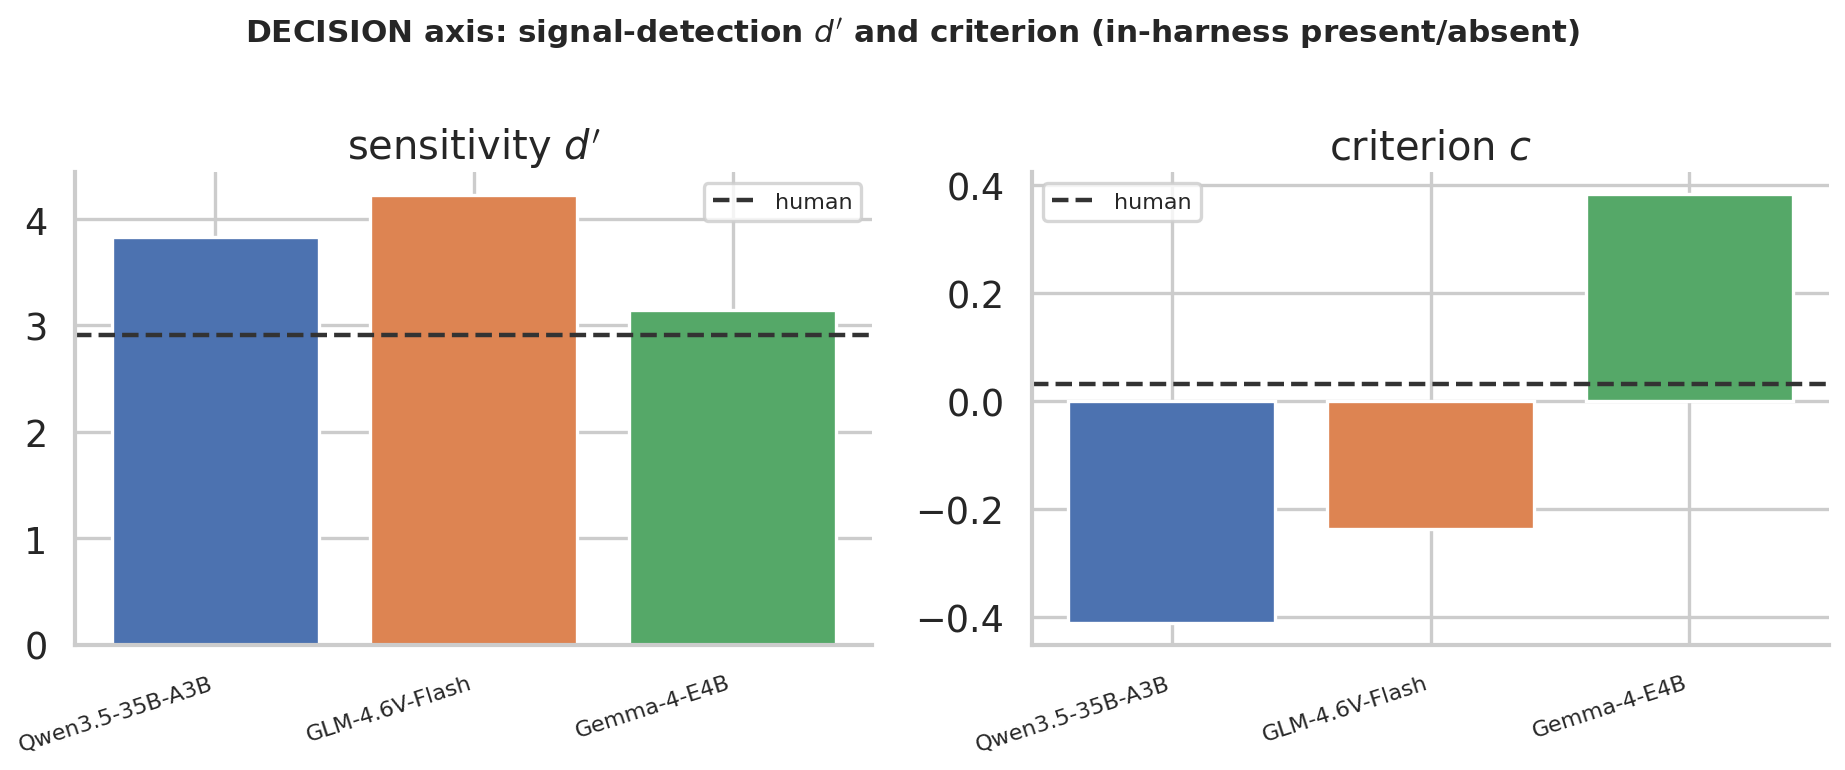
\includegraphics[width=0.84\linewidth]{figures/fig_decision.png}
\caption{Signal-detection sensitivity ($d'$) and criterion ($c$) for the in-harness present/absent
decision, per model against the human reference.}\label{fig:dec}\end{figure}
 
All three models detect targets near ceiling (target-present existence accuracy
\QwenTPexist/\GlmTPexist/\GemmaTPexist) with a comparable false-positive bias on absent scenes
(\QwenYesBias/\GlmYesBias/\GemmaYesBias), so subsequent search divergences cannot be attributed to
detection failure and the existence-passed sets are comparable across models. In the agentic task the
present/absent decision is highly sensitive for every model ($d'$
\QwenGPDprime/\GlmGPDprime/\GemmaGPDprime, against the human \HumanDprime), establishing that the
\emph{decision} axis is human-or-better. Model $d'$ is elicited from the agentic \textsc{found}/\textsc{absent} terminations and human $d'$ from the recorded gamepad response; this is a deliberate elicitation asymmetry rather than a confound, as both index the same present/absent judgment. Spatial targeting is measured in-harness (Sec.~\ref{sec:finding}), where the coordinate convention is fixed in the prompt; the resulting first-saccade rate is corroborated by high eventual success (TFP-end \QwenGPTFPend/\GlmGPTFPend/\GemmaGPTFPend) and low median fixation counts (\QwenGPNumFixTP/\GlmGPNumFixTP/\GemmaGPNumFixTP), and is stable across hit tolerances (Table~\ref{tab:tol}), so it is not an artefact of coordinate parsing.
 
 
%================================================================ Finding
\section{Finding axis}\label{sec:finding}
\begin{table}[ht]\centering
\caption{Outcome by foveation condition; each entry is Qwen / GLM / Gemma against the human reference
(first row). TFP@1 and TFP-end follow Eq.~\eqref{eq:tfp}; NumFix entries are per-group medians; the
last two columns give target-absent declared-absent rate and fixation-density CC with the human map.}
\label{tab:outcome}
\setlength{\tabcolsep}{4pt}
\resizebox{\linewidth}{!}{\begin{tabular}{l *{18}{c}}
\toprule
& \multicolumn{3}{c}{TFP@1} & \multicolumn{3}{c}{TFP-end} & \multicolumn{3}{c}{NFix-TP}
& \multicolumn{3}{c}{NFix-TA} & \multicolumn{3}{c}{TA decl.-abs} & \multicolumn{3}{c}{dens.\ CC} \\
\cmidrule(lr){2-4}\cmidrule(lr){5-7}\cmidrule(lr){8-10}\cmidrule(lr){11-13}\cmidrule(lr){14-16}\cmidrule(lr){17-19}
condition & Q & G & Gm & Q & G & Gm & Q & G & Gm & Q & G & Gm & Q & G & Gm & Q & G & Gm \\
\midrule
\textbf{human} & \multicolumn{3}{c}{\textbf{0.49}} & \multicolumn{3}{c}{\textbf{0.93}}
& \multicolumn{3}{c}{\textbf{3}} & \multicolumn{3}{c}{\textbf{5}}
& \multicolumn{3}{c}{---} & \multicolumn{3}{c}{---} \\
\midrule
sharp                  & 0.97 & 0.97 & 0.80 & 0.97 & 0.98 & 0.93 & 2 & 2 & 3 & 1 & 4 & 6 & 0.94 & 0.91 & 0.96 & 0.55 & 0.54 & 0.49 \\
\textbf{GP} & 0.97 & 0.97 & 0.80 & 0.98 & 0.98 & 0.93 & 2 & 2 & 3 & 1 & 4 & 5 & 0.93 & 0.91 & 0.96 & 0.58 & 0.63 & 0.50 \\
k8                     & 0.93 & 0.84 & 0.64 & 0.95 & 0.89 & 0.86 & 3 & 2 & 3 & 2 & 4 & 6 & 0.84 & 0.77 & 0.81 & 0.65 & 0.45 & 0.26 \\
k16                    & 0.78 & 0.71 & 0.42 & 0.91 & 0.80 & 0.75 & 3 & 3 & 4 & 4 & 4 & 6 & 0.78 & 0.77 & 0.68 & 0.70 & 0.38 & 0.45 \\
k24                    & 0.56 & 0.49 & 0.28 & 0.81 & 0.65 & 0.65 & 3 & 3 & 6 & 6 & 4 & 6 & 0.72 & 0.68 & 0.58 & 0.74 & 0.46 & 0.29 \\
k32                    & 0.42 & 0.33 & 0.19 & 0.71 & 0.53 & 0.59 & 3 & 3 & 6 & 7 & 4.5 & 7 & 0.62 & 0.65 & 0.52 & 0.70 & 0.43 & 0.26 \\
k48                    & 0.28 & 0.18 & 0.10 & 0.56 & 0.36 & 0.47 & 5 & 4 & 6 & 7 & 4 & 7 & 0.46 & 0.65 & 0.54 & 0.49 & 0.33 & 0.25 \\
k128                   & 0.15 & 0.09 & 0.01 & 0.31 & 0.22 & 0.39 & 6 & 4 & 6 & 6 & 4 & 6 & 0.85 & 0.86 & 0.78 & 0.18 & 0.14 & 0.19 \\
crop                   & 0.04 & 0.04 & 0.00 & 0.20 & 0.11 & 0.16 & 3 & 3 & 5 & 2 & 3 & 5 & 0.68 & 0.50 & 0.67 & 0.25 & 0.11 & 0.15 \\
\bottomrule
\end{tabular}}
\end{table}
\begin{figure}[ht]\centering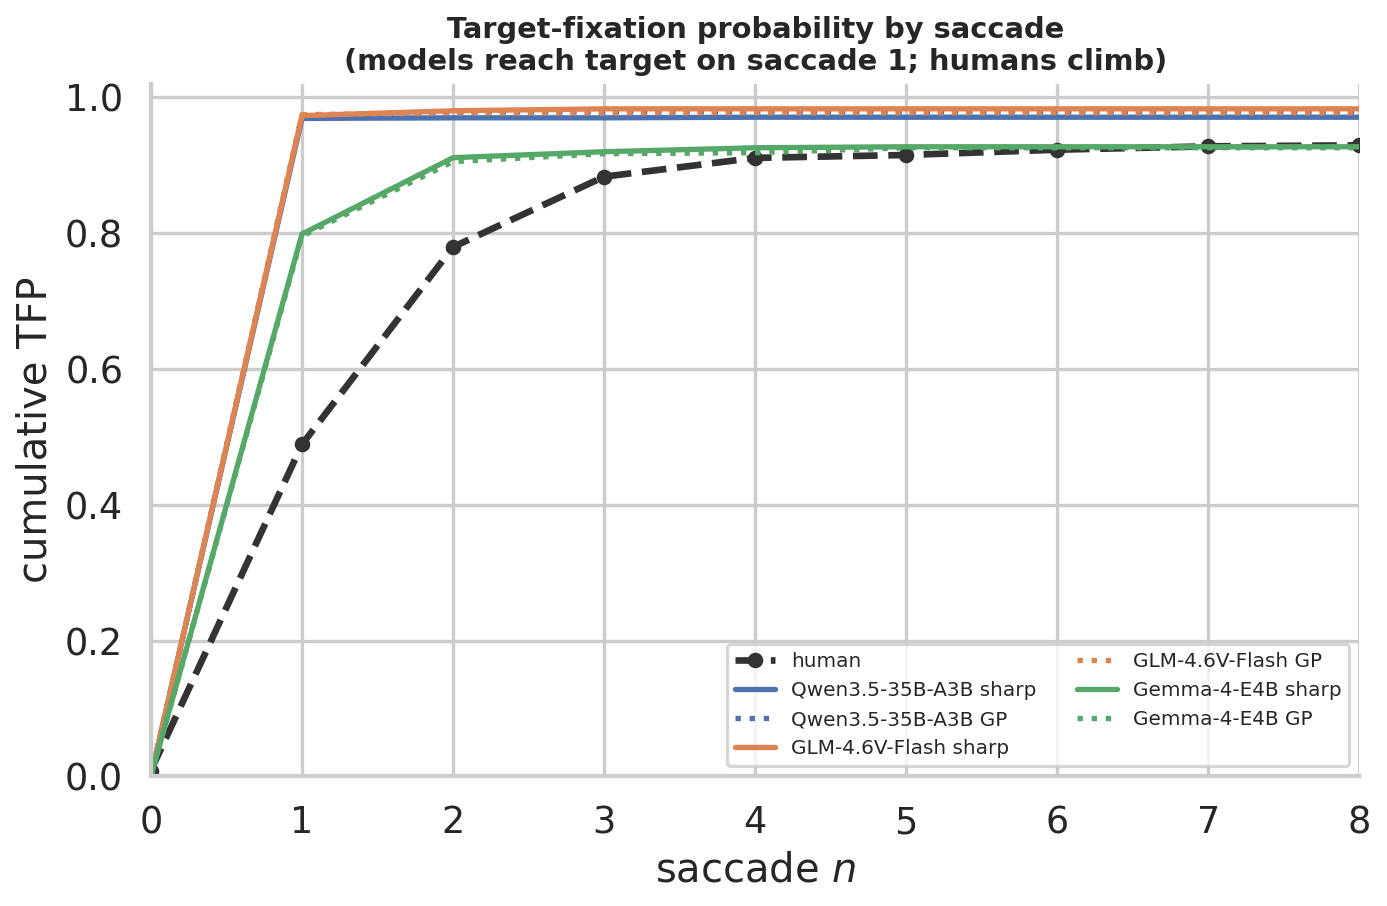
\includegraphics[width=0.68\linewidth]{figures/fig_tfp_curves.png}
\caption{Cumulative target-fixation probability by saccade (Eq.~\eqref{eq:tfp}) under \textsc{sharp}
(solid) and the human-matched GP (dotted) for the three models, against humans (dashed). The models
reach the target on the first saccade; human probability accrues over several fixations.}\label{fig:tfpc}\end{figure}
 
Under the human-matched condition every model fixates the target on the first saccade far more often than
humans (TFP@1 \QwenGPTFPone/\GlmGPTFPone/\GemmaGPTFPone\ versus \HumanTFPone) and reaches comparable
eventual success (TFP-end \QwenGPTFPend/\GlmGPTFPend/\GemmaGPTFPend\ versus \HumanTFPend), while issuing
no more fixations than humans (median NumFix \QwenGPNumFixTP/\GlmGPNumFixTP/\GemmaGPNumFixTP\ versus
\HumanNumFixTP). The advantage is therefore one of first-saccade efficiency rather than eventual
accuracy. Target-absent search extent varies across the three models: Qwen3.5-35B-A3B terminates after a single
fixation (median \QwenGPNumFixTA), GLM-4.6V-Flash searches longer (\GlmGPNumFixTA), and Gemma-4-E4B
searches to the human median (\GemmaGPNumFixTA\ versus \HumanNumFixTA). On the finding axis the models
are thus human-or-better throughout.
 
 
%================================================================ Gaze
\section{Gaze axis}\label{sec:gaze}
\begin{table}[ht]\centering
\caption{Intrinsic gaze signature: Cliff's $\delta$ against the human distribution (Eq.~\eqref{eq:cliffs};
$|\delta|>0.33$ in bold; sign is agent $-$ human) for every statistic and condition, for all three
models. Human medians: gaze entropy $1.58$ bits, saccade amplitude $8.57°$, refixation $0.00$, scanpath
length $19.4°$, center bias $10.0°$.}
\label{tab:signature}
\setlength{\tabcolsep}{4pt}\footnotesize
\resizebox{\linewidth}{!}{\begin{tabular}{llccccccc}
\toprule
model & condition & gaze entropy & saccade amp & refixation & scanpath len & center bias & turn angle & coverage \\
\midrule
Q & sharp & \textbf{$-$.68} & \textbf{$+$.52} & $+$.03 & $-$.27 & $-$.20 & $+$.03 & \textbf{$-$.75} \\
 & GP & \textbf{$-$.67} & \textbf{$+$.50} & $+$.04 & $-$.26 & $-$.18 & $+$.05 & \textbf{$-$.74} \\
 & k8 & \textbf{$-$.69} & $+$.20 & \textbf{$+$.36} & $-$.27 & $-$.05 & $+$.06 & \textbf{$-$.65} \\
 & k16 & \textbf{$-$.56} & $-$.03 & \textbf{$+$.49} & $-$.21 & $+$.01 & $+$.12 & \textbf{$-$.46} \\
 & k24 & \textbf{$-$.33} & $-$.08 & \textbf{$+$.52} & $-$.07 & $+$.02 & $+$.14 & $-$.18 \\
 & k32 & $-$.15 & $-$.07 & \textbf{$+$.50} & $+$.05 & $+$.00 & $+$.24 & $-$.03 \\
 & k48 & $+$.12 & $+$.01 & \textbf{$+$.54} & $+$.28 & $-$.04 & \textbf{$+$.45} & $+$.18 \\
 & k128 & $+$.33 & \textbf{$+$.73} & $+$.27 & \textbf{$+$.57} & $+$.17 & \textbf{$+$.67} & \textbf{$+$.46} \\
 & crop & $-$.24 & $+$.31 & $+$.26 & $-$.10 & \textbf{$-$.33} & \textbf{$+$.58} & $-$.11 \\
\midrule
G & sharp & \textbf{$-$.65} & \textbf{$+$.60} & $-$.12 & $-$.28 & $-$.29 & $-$.18 & \textbf{$-$.77} \\
 & GP & \textbf{$-$.65} & \textbf{$+$.61} & $-$.13 & $-$.28 & $-$.31 & $-$.21 & \textbf{$-$.77} \\
 & k8 & \textbf{$-$.65} & \textbf{$+$.43} & $+$.08 & $-$.28 & $-$.21 & $-$.06 & \textbf{$-$.71} \\
 & k16 & \textbf{$-$.53} & $+$.20 & $+$.30 & $-$.17 & $-$.05 & $+$.17 & \textbf{$-$.50} \\
 & k24 & \textbf{$-$.41} & $+$.02 & \textbf{$+$.45} & $-$.06 & $-$.02 & $+$.16 & \textbf{$-$.34} \\
 & k32 & $-$.26 & $-$.04 & \textbf{$+$.49} & $+$.07 & $-$.05 & $+$.19 & $-$.17 \\
 & k48 & $-$.10 & $-$.03 & \textbf{$+$.52} & $+$.25 & $+$.00 & $+$.19 & $+$.06 \\
 & k128 & $+$.01 & \textbf{$+$.42} & \textbf{$+$.43} & \textbf{$+$.61} & $+$.14 & \textbf{$+$.38} & $+$.29 \\
 & crop & \textbf{$-$.51} & $-$.08 & \textbf{$+$.65} & $-$.06 & \textbf{$-$.35} & $+$.31 & \textbf{$-$.37} \\
\midrule
Gm & sharp & $-$.28 & $+$.24 & $+$.13 & $-$.00 & $+$.06 & $+$.19 & $-$.28 \\
 & GP & $-$.27 & $+$.23 & $+$.13 & $+$.00 & $+$.06 & $+$.19 & $-$.26 \\
 & k8 & $-$.10 & $+$.01 & $+$.31 & $+$.14 & $+$.27 & $+$.24 & $+$.00 \\
 & k16 & $+$.19 & $+$.07 & $+$.27 & \textbf{$+$.35} & $+$.24 & $+$.30 & $+$.27 \\
 & k24 & \textbf{$+$.36} & $+$.16 & \textbf{$+$.38} & \textbf{$+$.56} & $+$.19 & \textbf{$+$.40} & \textbf{$+$.49} \\
 & k32 & \textbf{$+$.49} & $+$.20 & \textbf{$+$.41} & \textbf{$+$.66} & $+$.11 & \textbf{$+$.45} & \textbf{$+$.61} \\
 & k48 & \textbf{$+$.60} & $+$.30 & \textbf{$+$.45} & \textbf{$+$.76} & $-$.00 & \textbf{$+$.56} & \textbf{$+$.69} \\
 & k128 & \textbf{$+$.70} & \textbf{$+$.52} & \textbf{$+$.44} & \textbf{$+$.88} & $+$.02 & \textbf{$+$.62} & \textbf{$+$.82} \\
 & crop & $-$.08 & $+$.09 & \textbf{$+$.70} & \textbf{$+$.42} & $-$.19 & \textbf{$+$.48} & $+$.07 \\
\bottomrule
\end{tabular}
}
\end{table}
\begin{figure}[ht]\centering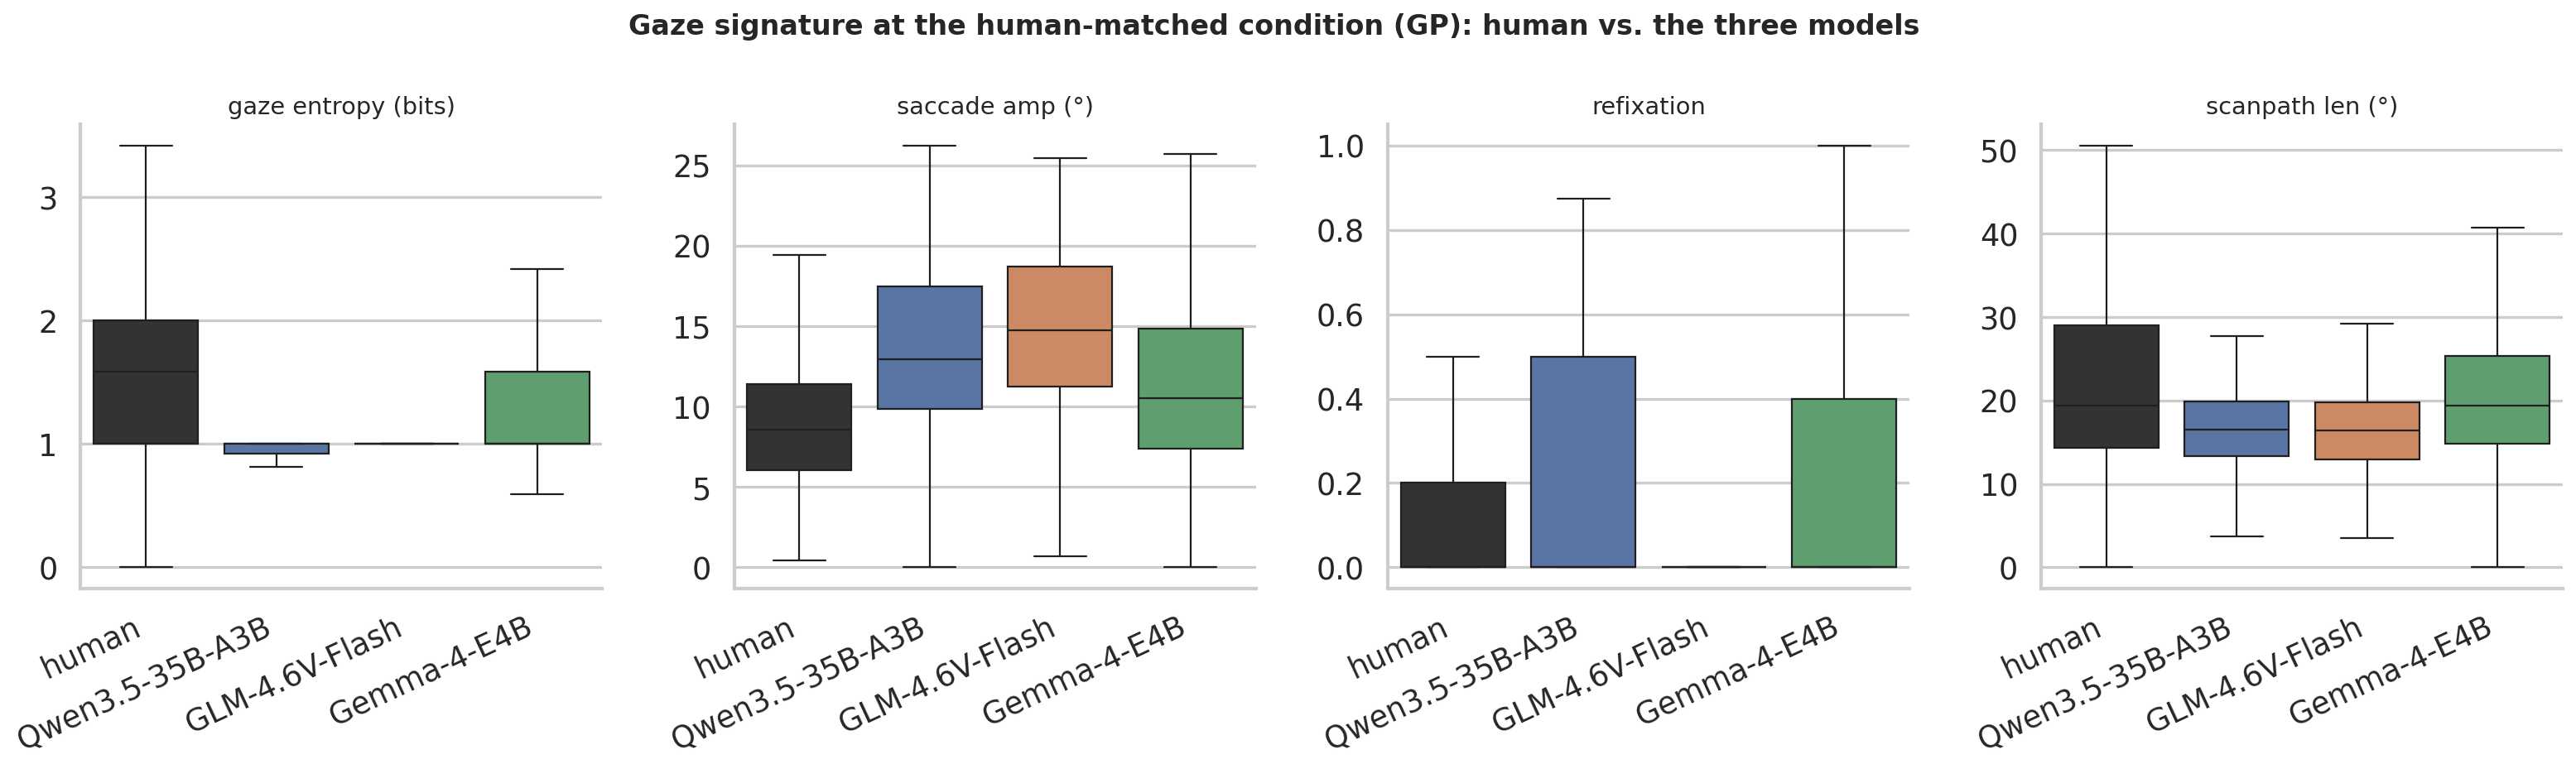
\includegraphics[width=\linewidth]{figures/fig_signature.png}
\caption{Per-scanpath gaze-statistic distributions at the human-matched condition, human against the
three models. The reasoning-tuned models concentrate gaze (low entropy) and make large saccades; Gemma-4-E4B
lies closest to the human distribution on the entropy, amplitude and scanpath-length panels (Qwen3.5-35B-A3B is closest on refixation).}\label{fig:sig}\end{figure}
 
Where outcomes coincide with humans, the eye-movement process does not, and the deviation is in the same
direction for all three models: gaze entropy lies below the human value (Cliff's $\delta$
\QwenGPEntropyD/\GlmGPEntropyD/\GemmaGPEntropyD), indicating spatially concentrated sampling, and saccade
amplitudes exceed it (\QwenGPSaccD/\GlmGPSaccD/\GemmaGPSaccD), indicating direct jumps to the target. The
magnitude of the deviation varies across the three models, with Gemma-4-E4B's effects roughly half
those of the two reasoning-tuned models, but the sign is invariant, so the signature is shared rather than
idiosyncratic. The directional and turning-angle distributions (Fig.~\ref{fig:dirturn}) corroborate this
characterisation and show that it does not depend on the choice of summary statistic.
 
\begin{figure}[ht]
  \begin{subfigure}{\linewidth}\centering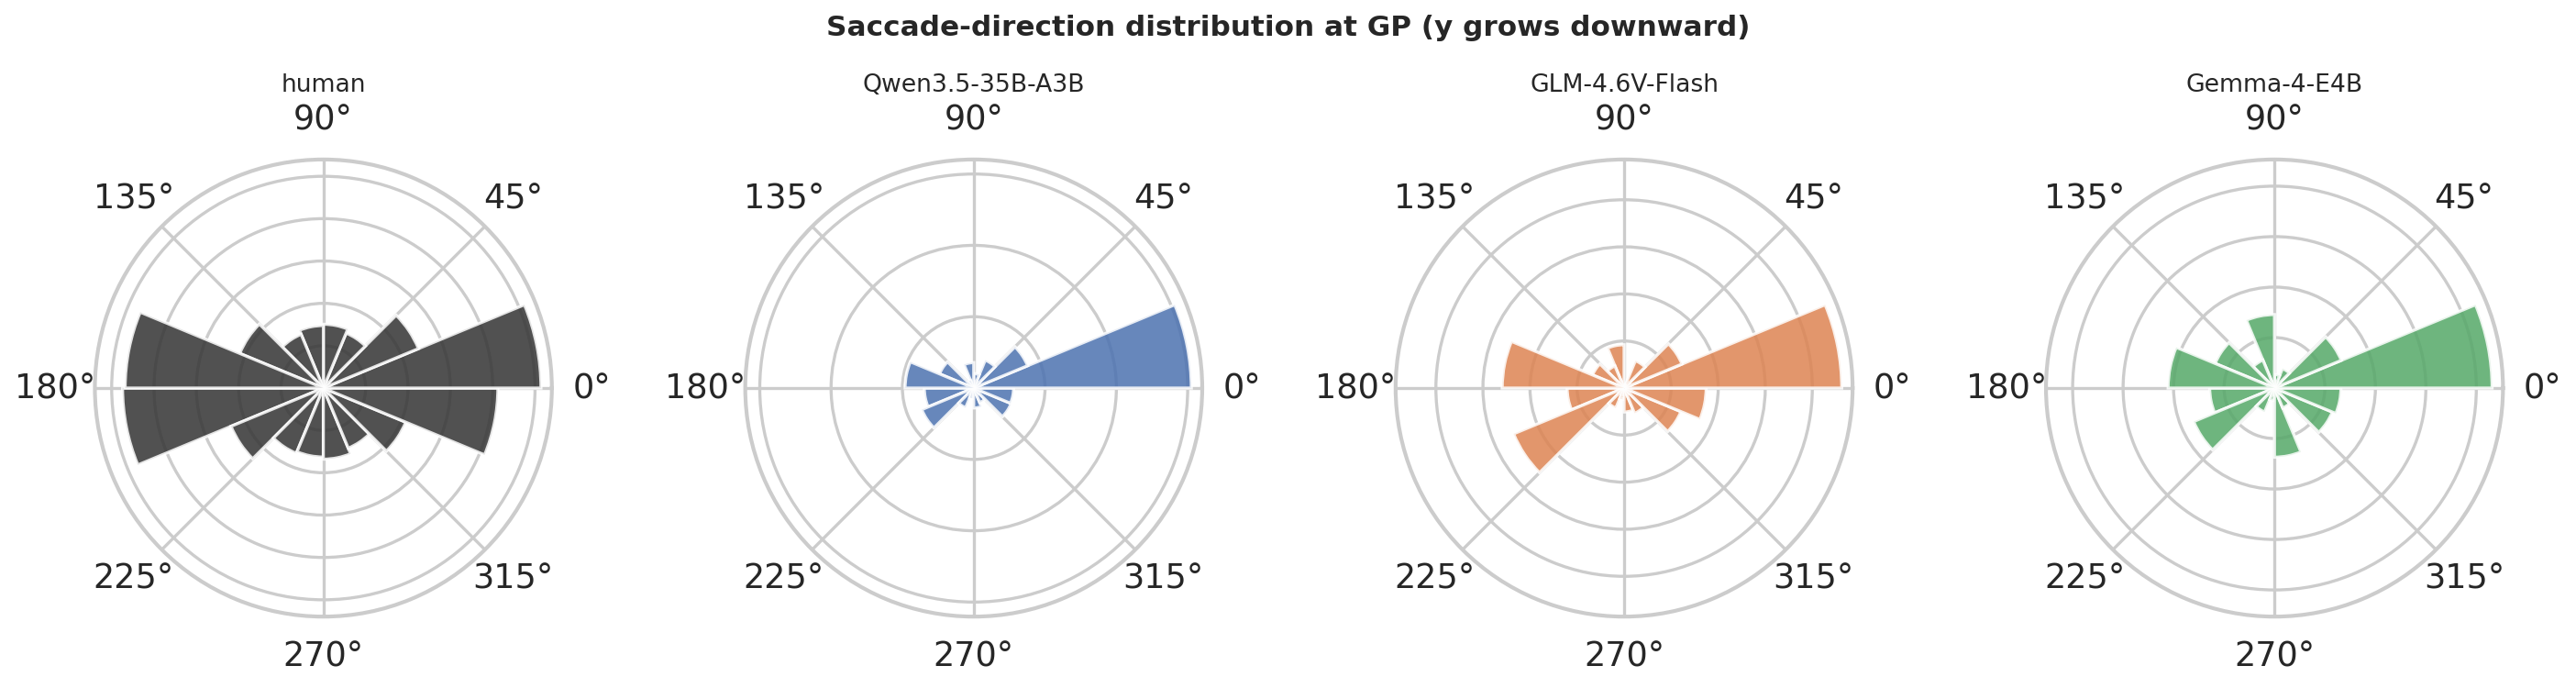
\includegraphics[width=0.82\linewidth]{figures/fig_polar.png}\caption{}\label{fig:polar}\end{subfigure}

  \begin{subfigure}{\linewidth}\centering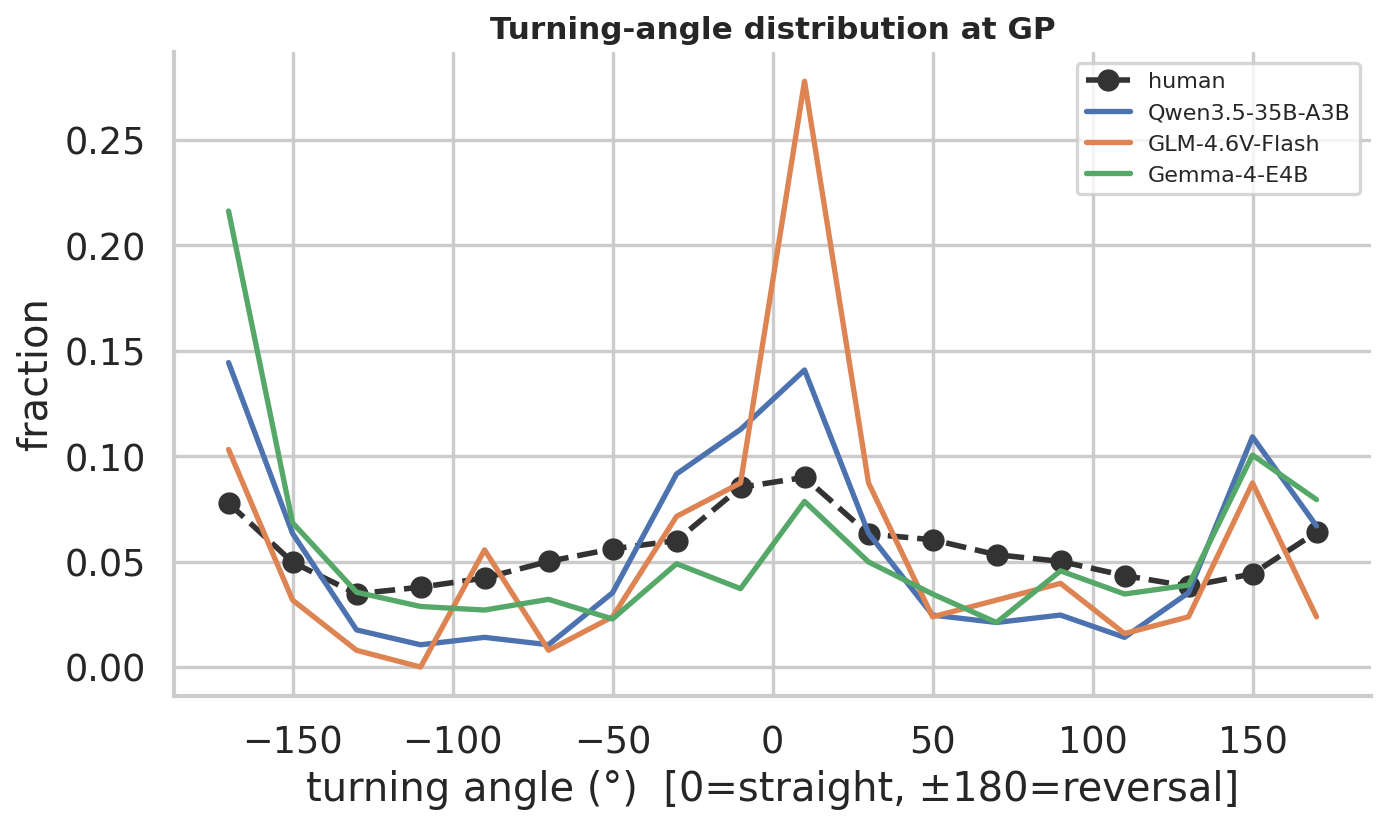
\includegraphics[width=0.82\linewidth]{figures/fig_turn.png}\caption{}\label{fig:turn}\end{subfigure}
  \caption{Distribution of (\subref{fig:polar}) saccade directions and (\subref{fig:turn}) turning angles
  at the human-matched condition. The models' directional and meander structure departs from the human
  reference, consistent with the entropy and amplitude effects.}\label{fig:dirturn}
\end{figure}
 
\begin{table}[ht]\centering
\caption{Scanpath similarity (ScanMatch, Sec.~\ref{sec:m-sim}) by condition: agent$\leftrightarrow$human
(AH) and agent$\leftrightarrow$agent (AA, cross-seed determinism) for each model. The
human$\leftrightarrow$human agreement ceiling is \HumanCeiling.}
\label{tab:similarity}
\setlength{\tabcolsep}{4pt}\small
\resizebox{\linewidth}{!}{\begin{tabular}{lcccccc}
\toprule
 & \multicolumn{2}{c}{Qwen3.5-35B-A3B} & \multicolumn{2}{c}{GLM-4.6V-Flash} & \multicolumn{2}{c}{Gemma-4-E4B} \\
condition & AH & AA & AH & AA & AH & AA \\
\midrule
\textbf{human ceiling} & \multicolumn{6}{c}{\textbf{0.53}} \\
sharp & 0.500 & 0.839 & 0.484 & 0.903 & 0.473 & 0.712 \\
GP & 0.505 & 0.843 & 0.485 & 0.913 & 0.469 & 0.713 \\
k8 & 0.527 & 0.814 & 0.491 & 0.868 & 0.462 & 0.697 \\
k16 & 0.521 & 0.776 & 0.476 & 0.800 & 0.405 & 0.594 \\
k24 & 0.479 & 0.696 & 0.445 & 0.712 & 0.324 & 0.477 \\
k32 & 0.420 & 0.597 & 0.402 & 0.613 & 0.275 & 0.424 \\
k48 & 0.332 & 0.499 & 0.320 & 0.495 & 0.240 & 0.373 \\
k128 & 0.244 & 0.407 & 0.266 & 0.423 & 0.217 & 0.397 \\
crop & 0.246 & 0.484 & 0.275 & 0.528 & 0.218 & 0.459 \\
\bottomrule
\end{tabular}
}
\end{table}
 
Cross-seed self-consistency exceeds the inter-observer ceiling for every model and follows the same
ordering as the intrinsic signature (agent$\leftrightarrow$agent ScanMatch
\QwenGPSelfConsist/\GlmGPSelfConsist/\GemmaGPSelfConsist\ versus the \HumanCeiling\ ceiling): each model
reproduces its own scanpath far more closely than two humans agree, Gemma-4-E4B least so.
Agent$\leftrightarrow$human similarity remains at or below the ceiling, so no model is more similar to a
human than two humans are to each other.
 
 
%================================================================ Multivariate
\section{Multivariate structure of the gaze signature}\label{sec:pca}
\begin{table}[ht]\centering
\caption{Principal components of the standardised five-statistic gaze signature across all groups, with
the loadings that render the axes interpretable.}
\label{tab:pca}\begin{tabular}{lcl}
\toprule
component & variance & dominant loadings \\
\midrule
PC1 & 45\% & $+0.62$ gaze entropy, $+0.62$ scanpath len, $+0.41$ center bias \\
PC2 & 30\% & $+0.69$ saccade amp, $-0.63$ refixation, $-0.35$ center bias \\
\bottomrule
\end{tabular}

\end{table}
 
A principal-component analysis of the per-group median signature vectors reduces the five statistics to
two interpretable axes (Table~\ref{tab:pca}); the leading component combines exploration extent
(scanpath length and gaze entropy) and the second contrasts saccade amplitude against refixation. In this
space every model, under every legible condition, occupies a region disjoint from the human reference
(main Fig.~3b), approaching it only under degradation severe enough that the target is no longer found.
That three architecturally distinct models from three families share this region is the multivariate
expression of the gaze divergence.
 
 
%================================================================ Mechanism
\section{Mechanism of the divergence}\label{sec:mech}
 
\paragraph{The divergence is consistent with a single-pass architecture rather than an acuity effect.}
The human-matched condition is behaviourally indistinguishable from no foveation for every model and
statistic, even though it measurably degrades the periphery (Fig.~\ref{fig:gps}; e.g.\ first-saccade
targeting \QwenGPTFPone\ under GP versus \QwenSharpTFPone\ under \textsc{sharp}). A parallel vision encoder
resolves a legible frame in a single pass and saccades directly to the target; matching the retinal
\emph{input} therefore does not reconstruct the serial sampling constraint that produces human search.
 
\begin{figure}[ht]\centering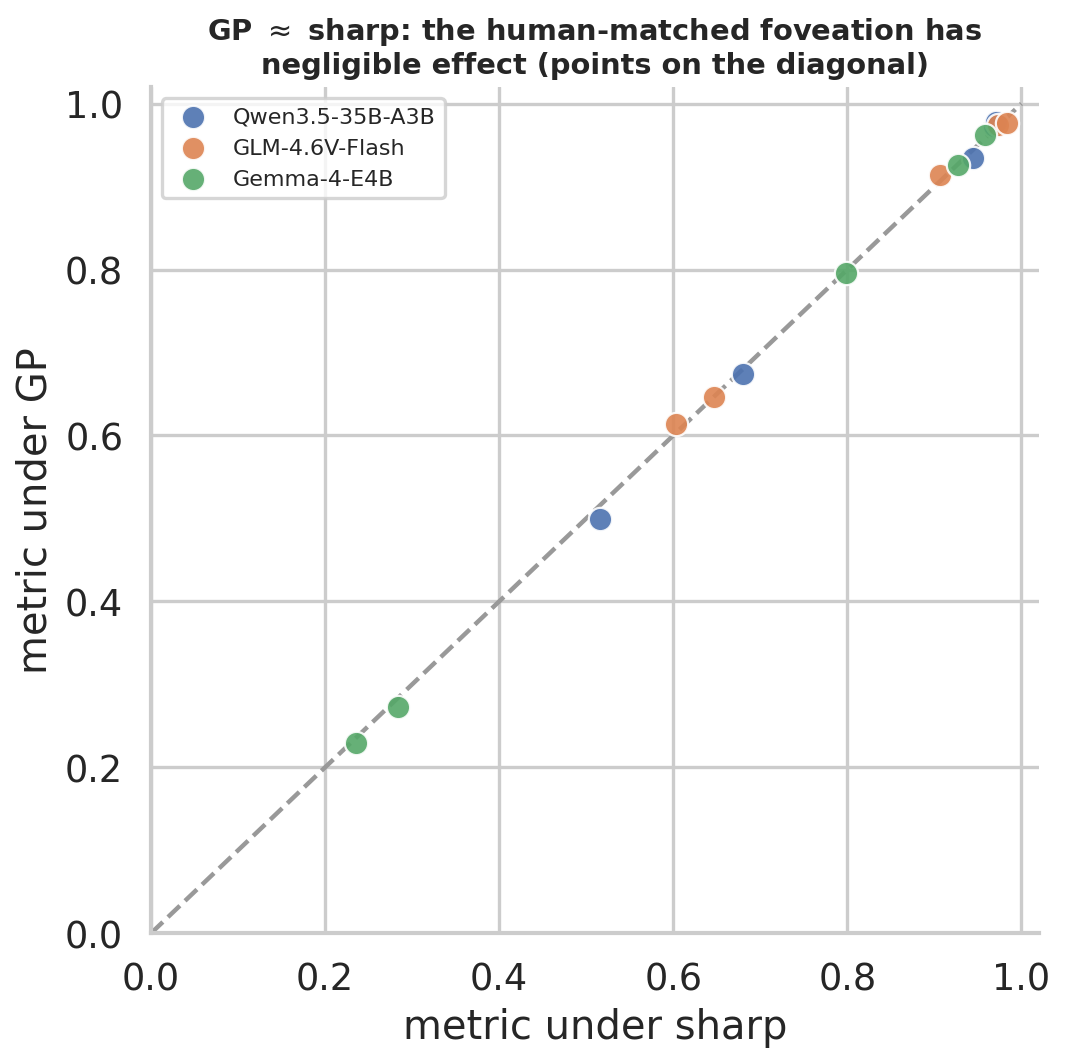
\includegraphics[width=0.56\linewidth]{figures/fig_gp_sharp.png}
\caption{Each statistic under \textsc{sharp} (abscissa) versus the human-matched GP condition (ordinate),
per model. Points lie on the identity line: the human-matched foveation changes behaviour negligibly.}\label{fig:gps}\end{figure}
 
\paragraph{The matched property is spatial; the divergent property is temporal.}
The models' spatial prior is approximately human: center bias is statistically indistinguishable from the
human value (sub-threshold $\delta$ in Table~\ref{tab:signature}) and fixation density correlates
positively with the human map (CC \QwenGPDensityCC/\GlmGPDensityCC/\GemmaGPDensityCC; full agreement measures in Table~\ref{tab:density}), so the models look
in broadly human-relevant places. What differs is the temporal organisation of looking: the order,
amplitude and determinism of fixations (Fig.~\ref{fig:spt}). The missing component is serial sampling,
not the spatial prior.

\begin{table}[ht]\centering
\caption{Fixation-density agreement with the human map (Sec.~\ref{sec:m-dens}) under \textsc{sharp} and the human-matched condition: linear correlation CC, normalised scanpath saliency NSS, and Kullback--Leibler divergence KL. CC and NSS (higher is closer) are highest for GLM-4.6V-Flash; KL (lower is closer) is lowest for Gemma-4-E4B. All three models correlate positively with the human map.}
\label{tab:density}
\begin{tabular}{lcccccc}
\toprule
 & \multicolumn{3}{c}{\textsc{sharp}} & \multicolumn{3}{c}{\textsc{geisler--perry}} \\
\cmidrule(lr){2-4}\cmidrule(lr){5-7}
model & CC & NSS & KL & CC & NSS & KL \\
\midrule
Qwen3.5-35B-A3B & 0.55 & 0.57 & 1.39 & 0.58 & 0.60 & 1.30 \\
GLM-4.6V-Flash  & 0.54 & 0.54 & 1.19 & 0.63 & 0.63 & 0.74 \\
Gemma-4-E4B     & 0.49 & 0.48 & 0.47 & 0.50 & 0.48 & 0.46 \\
\bottomrule
\end{tabular}

\end{table}
 
\begin{figure}[ht]\centering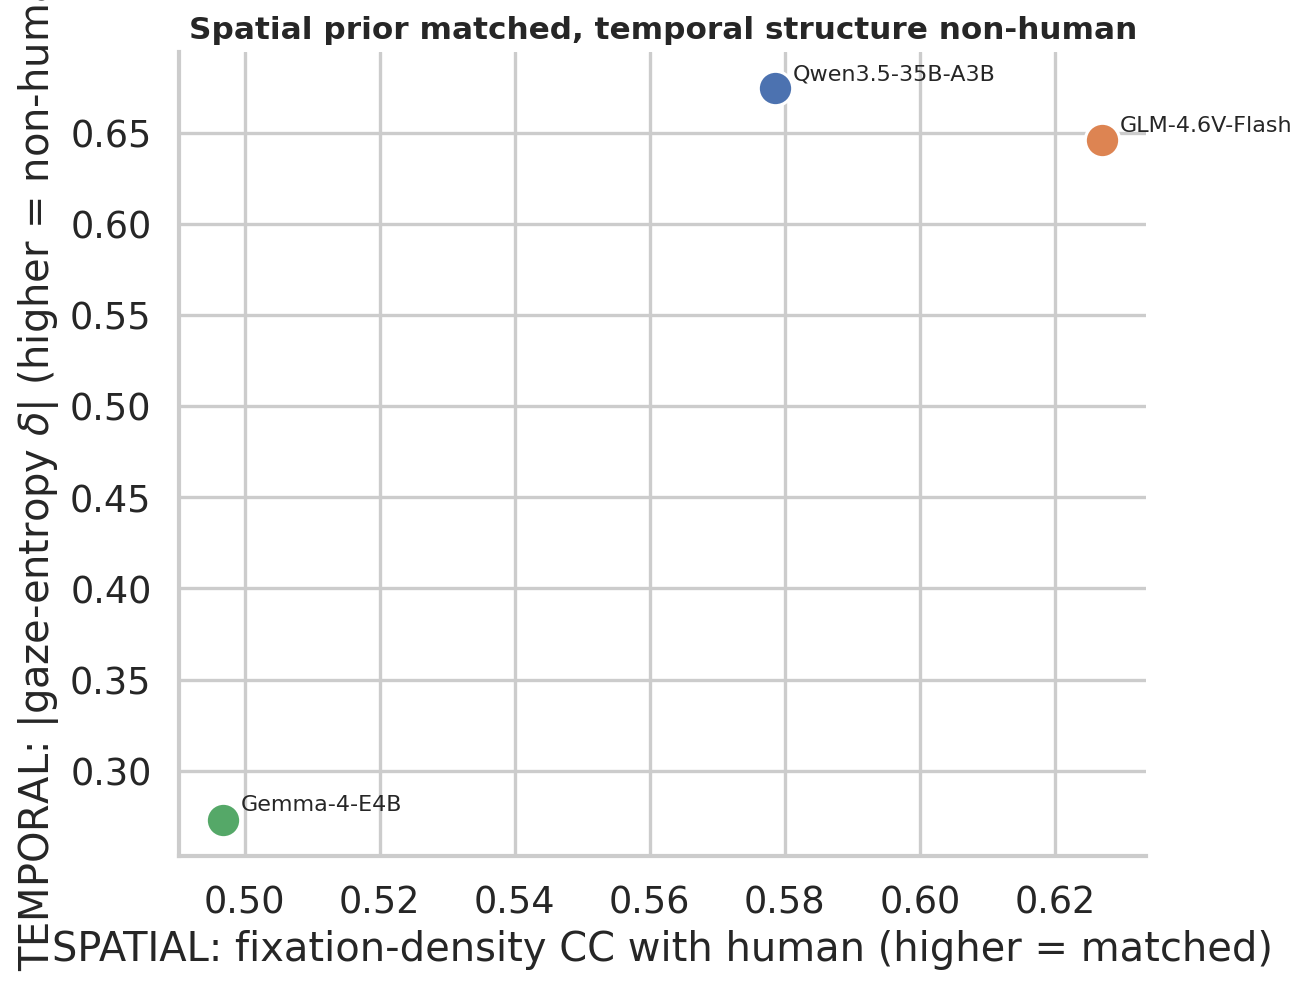
\includegraphics[width=0.6\linewidth]{figures/fig_spatial_temporal.png}
\caption{Spatial agreement with humans (fixation-density CC, abscissa) against temporal divergence
(absolute gaze-entropy effect, ordinate). The models match \emph{where} humans look while diverging in
\emph{how} the looking unfolds.}\label{fig:spt}\end{figure}
 
\paragraph{No degradation regime recovers human-like search.}
Sweeping the synthetic degradation does not produce a regime that is simultaneously human-like in
first-saccade targeting and in eventual success (Fig.~\ref{fig:gistS}): the two quantities decline
together. At the degradation level that lowers first-saccade targeting to the human rate
(\HumanTFPone), namely $k{=}32$ for Qwen3.5-35B-A3B and $k{=}16$ for Gemma-4-E4B, eventual success has
already fallen well below the human level (TFP-end \QwenKthirtytwoTFPend\ and \GemmaKsixteenTFPend\
respectively). There is no operating point at which the models search like humans and still find the
target.
 
\begin{figure}[ht]\centering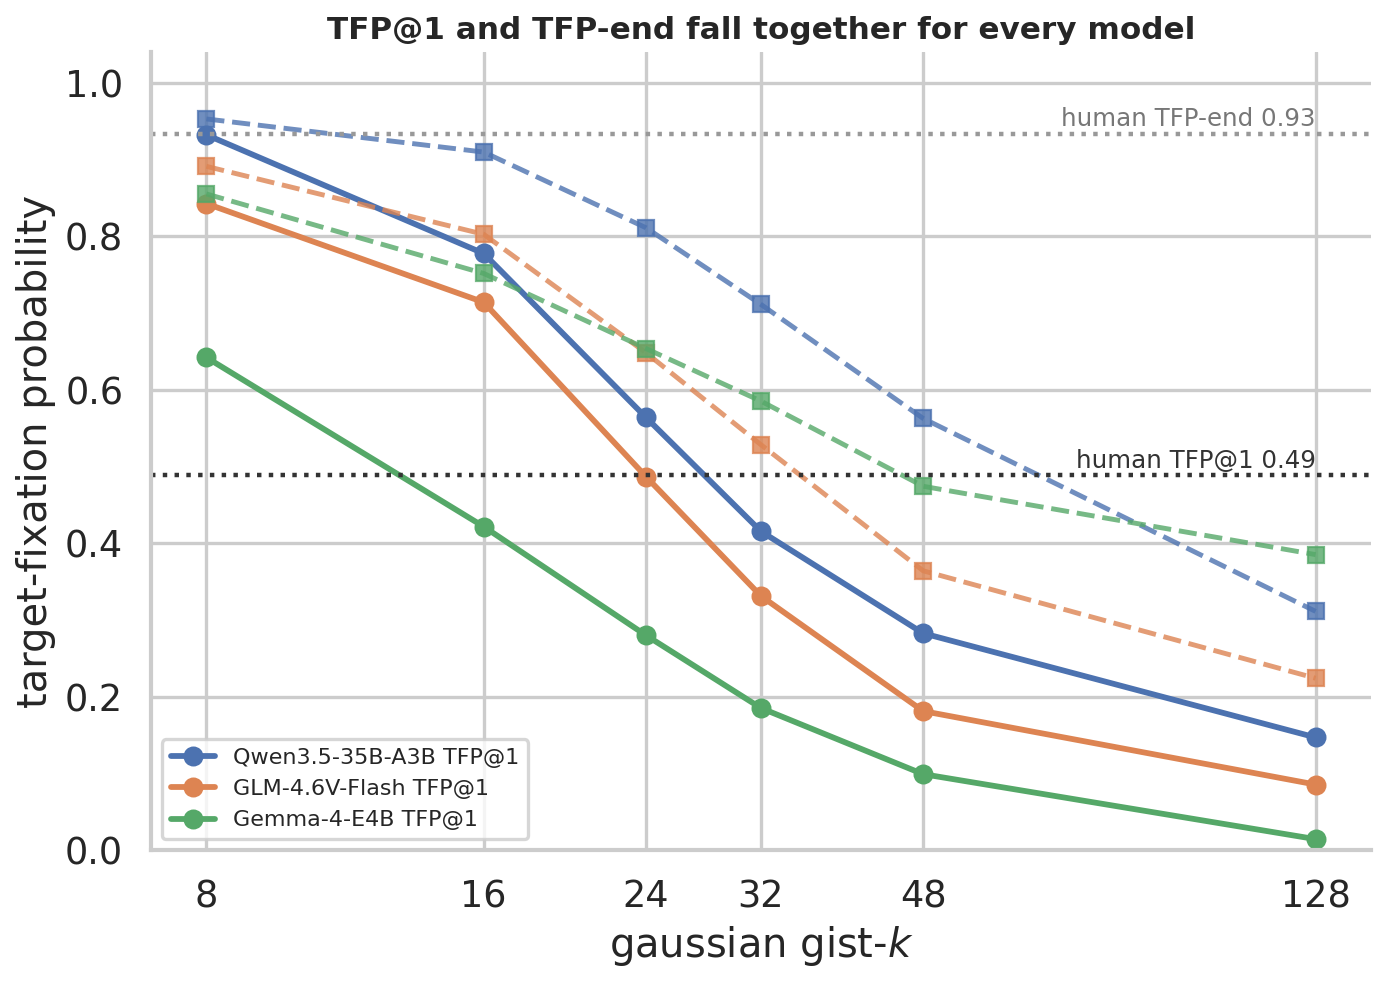
\includegraphics[width=0.66\linewidth]{figures/fig_gist.png}
\caption{First-saccade targeting (solid) and eventual success (dashed) as functions of the synthetic
degradation factor $k$, for the three models, with human reference levels. The two curves fall together;
no $k$ yields human-like search at human-like success.}\label{fig:gistS}\end{figure}
 
\paragraph{Failure mode under vanishing evidence.}
As the periphery is degraded the models do not lengthen their search in a graceful, human-like manner.
Refixation first rises as cells are revisited, and at the most severe degradation the target-absent
declared-absent rate rebounds as the models default to an ``absent'' response
(Fig.~\ref{fig:thr}). Because one clause of the prompt encourages the use of glimpse memory, the absolute
refixation level is in part prompt-shaped; the failure signature is the trend across degradation, not its
absolute value. This pattern, rising refixation followed by default-absent termination, is model-internal and requires no human reference to detect.
 
\begin{figure}[ht]\centering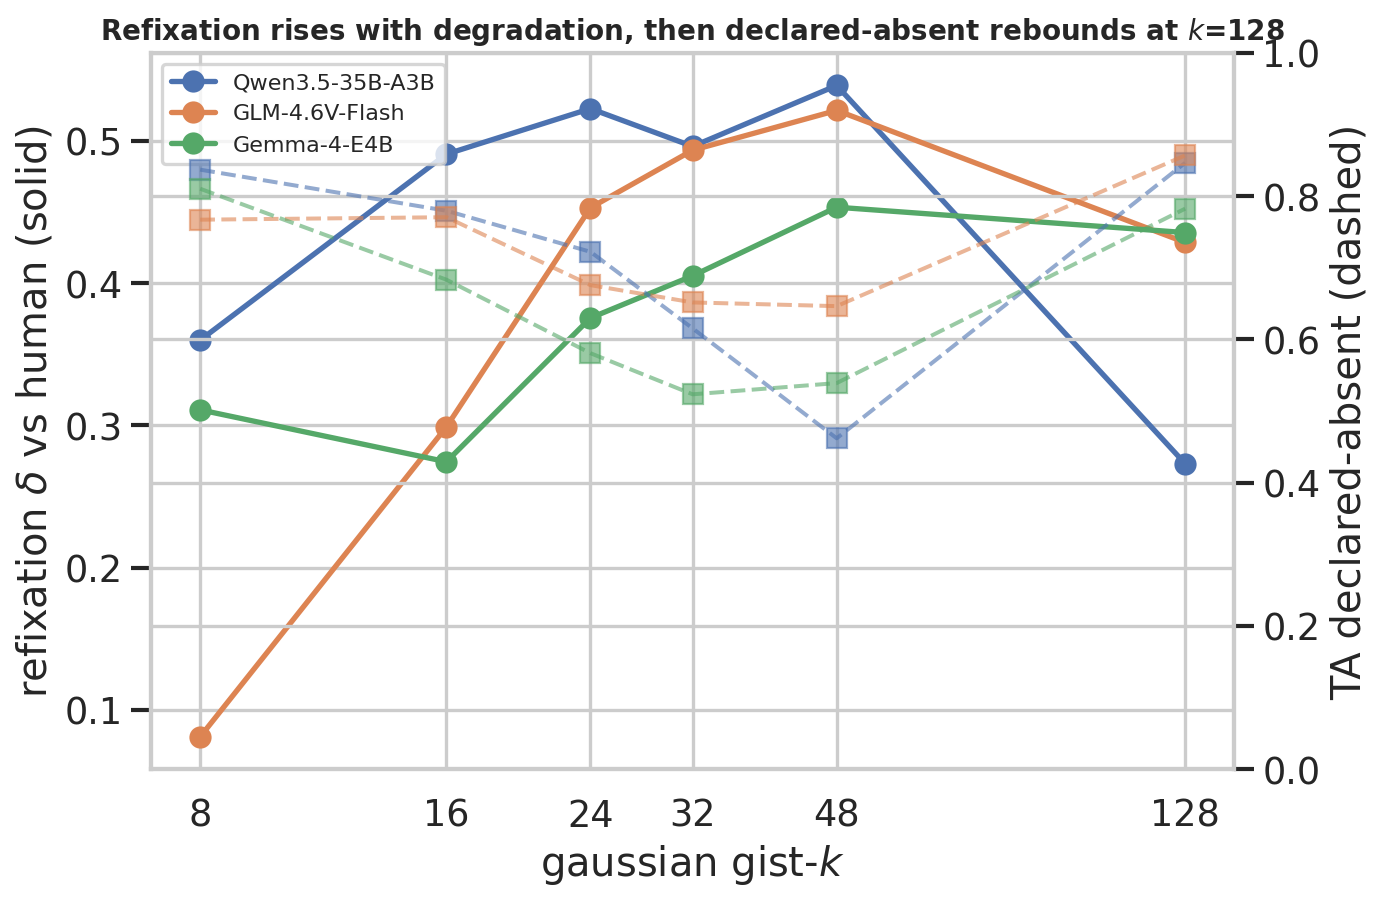
\includegraphics[width=0.66\linewidth]{figures/fig_thrash.png}
\caption{As degradation increases, the refixation effect (solid) rises (the models revisit locations) and
then the declared-absent rate (dashed) rebounds at the most severe degradation as the models
default to an absent response.}\label{fig:thr}\end{figure}
 
 
%================================================================ Robustness
\section{Robustness and cross-model variation}\label{sec:robust}
\begin{table}[ht]\centering
\caption{First-saccade targeting by eccentricity $\times$ target-size stratum (sharp), human against the
three models.}
\label{tab:strata}\begin{tabular}{lcc}
\toprule
stratum (n) & human TFP@1 & sharp TFP@1 (Q / G / Gm) \\
\midrule
near-small (44) & 0.54 & 0.96 / 0.97 / 0.76 \\
near-large (26) & 0.65 & 0.97 / 0.98 / 0.85 \\
far-small (26) & 0.37 & 1.00 / 0.98 / 0.64 \\
far-large (45) & 0.39 & 0.96 / 0.96 / 0.89 \\
\bottomrule
\end{tabular}

\end{table}
\begin{figure}[ht]\centering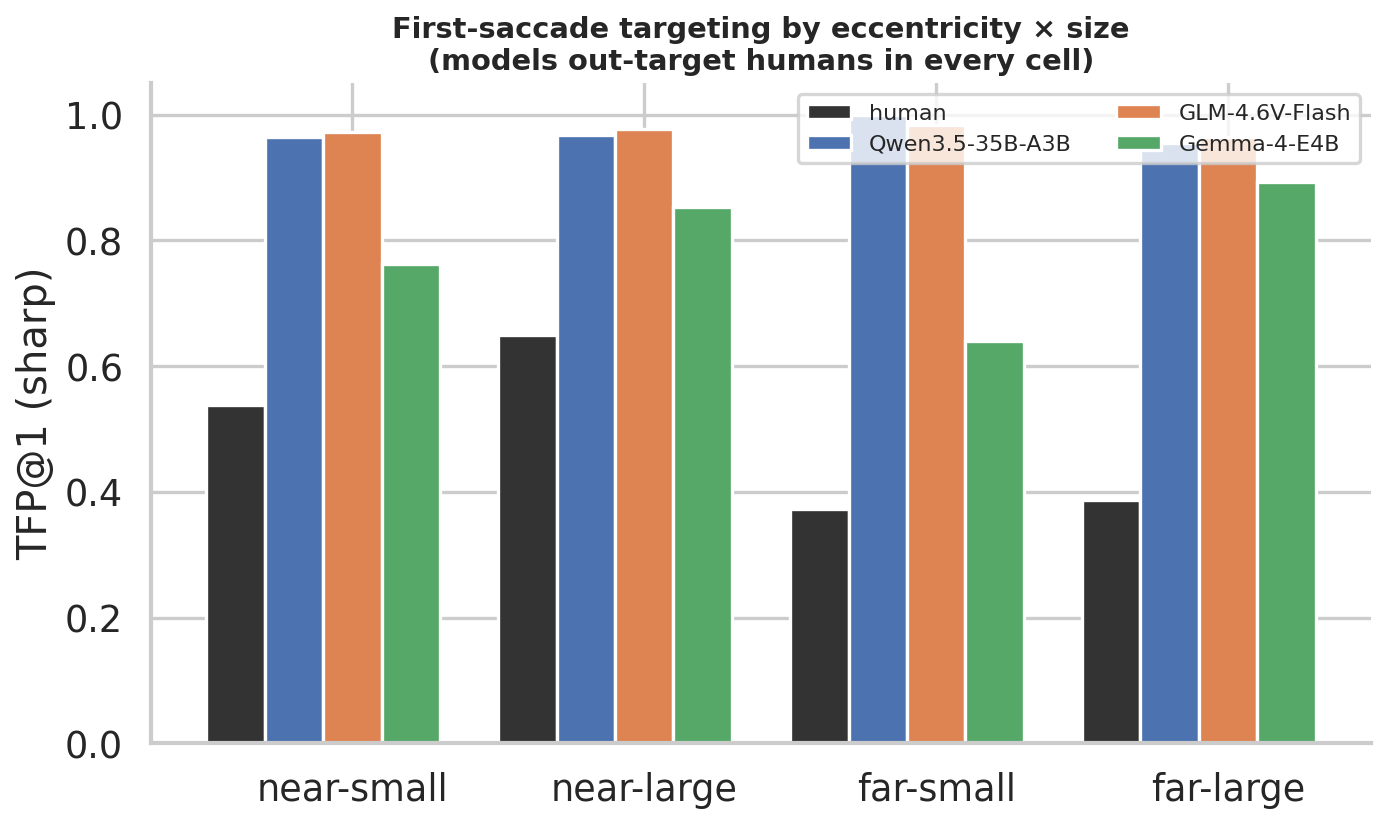
\includegraphics[width=0.6\linewidth]{figures/fig_stratum.png}
\caption{First-saccade targeting per difficulty stratum; the models exceed humans in every eccentricity
$\times$ size cell, including the hardest.}\label{fig:strat}\end{figure}
 
The first-saccade advantage is not an artifact of easy targets: it holds in every eccentricity $\times$
size stratum, including the hardest (Table~\ref{tab:strata}). It is likewise insensitive to the
target-box tolerance: recomputing TFP@1 at $\pm0.5°$, $\pm1°$ and $\pm1.5°$ shifts any value by at most
the amounts in Table~\ref{tab:tol}, and the model--human gap holds at every tolerance.
 
\begin{table}[ht]\centering
\caption{Maximum absolute change in TFP@1 across box tolerances of $0.5$, $1$ and $1.5$ degrees, per
model.}
\label{tab:tol}\begin{tabular}{lc}
\toprule
model & max $|\Delta$TFP@1$|$ over $\pm0.5/1/1.5°$ \\
\midrule
Qwen3.5-35B-A3B & 0.063 \\
GLM-4.6V-Flash & 0.076 \\
Gemma-4-E4B & 0.095 \\
\bottomrule
\end{tabular}

\end{table}
 
\begin{table}[ht]\centering
\caption{Linear mixed-effects fixed effects against the human reference (Eq.~\eqref{eq:lmm}; $\Delta$
[95\% CI]) under \textsc{sharp} and the human-matched condition, with crossed scene and rater random
intercepts. Bold indicates a confidence interval that excludes zero.}
\label{tab:mixed}\begin{tabular}{llcc}
\toprule
model & metric & sharp $\Delta$ [95\% CI] & GP $\Delta$ [95\% CI] \\
\midrule
Qwen3.5-35B-A3B & gaze entropy & \textbf{$-0.62$ [$-0.69,-0.56$]} & \textbf{$-0.61$ [$-0.67,-0.54$]} \\
 & saccade amp. & \textbf{$+4.57$ [$+3.19,+5.95$]} & \textbf{$+4.53$ [$+3.15,+5.91$]} \\
 & NumFix & \textbf{$-1.53$ [$-1.94,-1.13$]} & \textbf{$-1.49$ [$-1.89,-1.08$]} \\
 & TFP@1 & \textbf{$+0.47$ [$+0.40,+0.54$]} & \textbf{$+0.48$ [$+0.41,+0.55$]} \\
\midrule
GLM-4.6V-Flash & gaze entropy & \textbf{$-0.60$ [$-0.67,-0.52$]} & \textbf{$-0.60$ [$-0.67,-0.52$]} \\
 & saccade amp. & \textbf{$+5.58$ [$+4.84,+6.32$]} & \textbf{$+5.62$ [$+4.88,+6.35$]} \\
 & NumFix & \textbf{$-1.51$ [$-1.89,-1.13$]} & \textbf{$-1.60$ [$-1.98,-1.22$]} \\
 & TFP@1 & \textbf{$+0.48$ [$+0.40,+0.56$]} & \textbf{$+0.48$ [$+0.40,+0.56$]} \\
\midrule
Gemma-4-E4B & gaze entropy & \textbf{$-0.23$ [$-0.33,-0.14$]} & \textbf{$-0.22$ [$-0.31,-0.12$]} \\
 & saccade amp. & \textbf{$+2.17$ [$+1.34,+3.00$]} & \textbf{$+2.20$ [$+1.37,+3.03$]} \\
 & NumFix & $-0.26$ [$-0.78,+0.27$] & $-0.03$ [$-0.55,+0.49$] \\
 & TFP@1 & \textbf{$+0.31$ [$+0.19,+0.42$]} & \textbf{$+0.30$ [$+0.19,+0.41$]} \\
\bottomrule
\end{tabular}

\end{table}
 
\begin{figure}[ht]\centering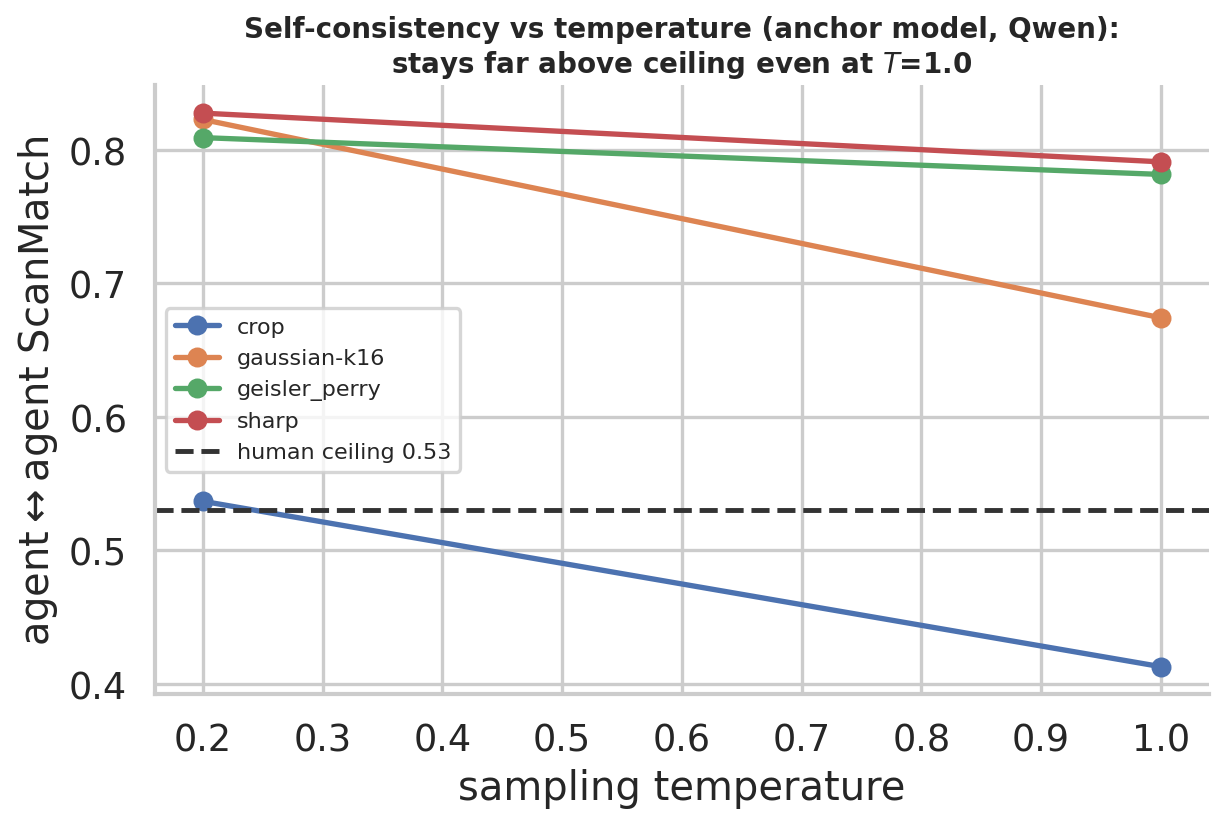
\includegraphics[width=0.6\linewidth]{figures/fig_temp.png}
\caption{Cross-seed self-consistency as a function of sampling temperature (anchor model, Qwen, core
conditions), against the human$\leftrightarrow$human ceiling \HumanCeiling.}\label{fig:temp}\end{figure}
 
The distributional effects survive the mixed-effects model of Eq.~\eqref{eq:lmm}, which controls for both
scene and rater (Table~\ref{tab:mixed}): the gaze-entropy, saccade-amplitude and first-saccade effects
have confidence intervals excluding zero for all three models. Two features of the cross-model ordering
are notable. First, Gemma-4-E4B's effects are the smallest on five of the seven gaze statistics (entropy, saccade
amplitude, scanpath length, center bias, coverage), making it the most human-like model overall; Qwen3.5-35B-A3B
is closest to humans on refixation and turning angle (Table~\ref{tab:signature}). Second, at the human-matched condition its search-extent effect is the single
fixed effect whose interval includes zero ($\Delta$\GemmaNumFixDelta), making its number of fixations
statistically indistinguishable from the human value. We interpret this ordering as a consequence of
weaker single-pass targeting (which forces additional, smaller, more variable fixations) rather than a
more human-like search strategy. The three models differ in architecture, training recipe (only
Gemma-4-E4B is not reasoning-tuned) and mixture-of-experts sparsity; these factors covary and cannot
be separated with three observations, so the ordering is reported descriptively. The high cross-seed
determinism is not an artifact of low-temperature decoding: in a temperature sweep on the anchor model (Qwen3.5-35B-A3B)
it remains well above the inter-observer ceiling even at temperature $1.0$ on the legible conditions
(Fig.~\ref{fig:temp}), and the deployed-temperature self-consistency of all three models
(Table~\ref{tab:similarity}) shows the same ordering.
 
 
%================================================================ Integrity
\section{Data completeness}\label{sec:integrity}
All three models completed the full design (\NImages\ scenes, \NSeeds\ seeds and nine conditions), with
no trials excluded from the final analysis. Two protocol details bear on the integrity of the records. GLM-4.6V-Flash's one-shot detection responses were re-collected after an initial server interruption, recovering
its detection ceiling without affecting its search records. Gemma-4-E4B emitted its terminal
present/absent decision in a coordinate format requiring canonical normalisation before parsing; the
affected episodes were reconstructed from their logged turn sequences, each verified to reproduce the
recorded gaze path up to the decision, and the residual truncated episodes were re-collected under the
identical protocol. Neither procedure altered the other models' records, and all reported quantities are
computed from the recorded scanpaths under the single set of definitions given in
Sec.~\ref{sec:metrics}.
 
 
%================================================================ Implications / scope
\section{Implications and scope}\label{sec:scope}
\paragraph{Evaluation metrics.} The dissociation has a direct methodological consequence. The models
match the human present/absent answer and partially match the human fixation-density map (CC
\QwenGPDensityCC/\GlmGPDensityCC/\GemmaGPDensityCC) while diverging on every temporal measure of the gaze
process. Because answer-alignment scores and single-shot saliency overlap are computed on outcomes or on
a time-collapsed spatial map, neither is sensitive to the axis on which the divergence occurs; a high
score on either is therefore necessary but not sufficient evidence of human-like vision, and certifying
process-level correspondence requires sequence-level, temporal measurement of the kind defined here.
 
\paragraph{Suitability as human-vision surrogates.} It follows that zero-shot multimodal models are
adequate surrogates for studies of \emph{outcome and spatial allocation} (detectability, approximate
region of interest, present/absent rates) and inadequate for studies of \emph{process and temporal
dynamics} (scanpath prediction, fixation counts and amplitudes, stopping behaviour, the time course of
evidence accumulation). Because the inadequacy is a shared property of the class rather than of any
instance, it is not removed by model selection within this family.
 
\paragraph{A null model for serial search.} Conversely, a system that attains human-or-better outcomes
\emph{without} a serial sampling bottleneck is a useful null model: contrasting a serial searcher (human
or model) against this parallel one-pass reference isolates the behaviours attributable to seriality
(eccentricity-dependent search cost, inspection-driven refixation, graded confirmatory stopping) from
those attributable to detection ability or spatial priors, which the null already reproduces.
 
\paragraph{Scope.} This study examined general-purpose models under a fixed foveation constraint. It did
not evaluate search-trained agentic models with learned zoom or tool-use policies, pointing-native or
frontier closed-source models, or an explicit probe of semantic guidance; nor did it run per-model
temperature sweeps beyond the anchor model. None of these bears on the three central findings, which
already hold across three distinct model families.

\clearpage
\section{Prompt}\label{sec:prompt}

\lstset{style=prompt}
\begin{lstlisting}
You are controlling a single eye that searches a photograph for a specific object.
You can only see clearly at the point you are currently looking; everything else is
blurred, with sharpness falling off the farther it is from your gaze, like human
peripheral vision. To inspect another region you must move your gaze there.

Each turn you receive the image as it currently looks from your gaze point. Earlier
turns show where you looked before and what you saw; use that history to decide where
to look next and to avoid re-checking the same spots.

Coordinates are normalized: x and y are each between 0.0 and 1.0. (0,0) is the
top-left corner, (1,1) the bottom-right; x grows rightward, y grows downward.

Your job is a PRESENT/ABSENT decision: is the target object in this image? On every turn
do exactly one of:
  - move your gaze to a new point to keep searching;
  - decide the target is PRESENT (FOUND): you can clearly see it at your gaze point;
  - decide the target is ABSENT: you are confident it is nowhere in the image.

Think briefly if you want, then end your reply with ONE directive line in EXACTLY one
of these forms and nothing after it:
  LOOK: x=<0..1>, y=<0..1>
  FOUND: x=<0..1>, y=<0..1>
  ABSENT
\end{lstlisting}



\bibliographystyle{splncs04}
\bibliography{main}

\end{document}
